\section{Background}\label{sec:background}
\label{sec:cast}
The Gauss-Bonnet Theorem states

\begin{theorem}[The Gauss-Bonnet Theorem] \label{thm:g-b}

$$\sum_{v\in V_{int}} K(v) + \sum_{v\in V_{\partial S}} k_g(v) = 2\pi \chi(S)$$
where $S$ is a triangulation, $K(v)$ is the discrete Gaussian curvature
of a vertex, $k_g(g)$ is the discrete geodesic curvature and
$\chi$ is the Euler characteristic.
\end{theorem}
In this section, we define these symbols.


\subsection{Simple Polygons}
\label{sec:warm-up}

Some of us may remember the following special case
of the Gauss-Bonnet theorem from middle school geometry.
An \EMPH{exterior angle} is created when we extend one of the sides of a polygon.
See \figref{exterior-angles} for an example.
The exterior angle at a vertex can be positive or negative.
If we traverse a polygon and add up the exterior angles
we get $2\pi$ because we perform one revolution.
This is a special case of the Gauss-Bonnet theorem.
No matter how we bend or stretch our polygon,
if the boundary of the polygon stays closed and simple,
the sum the exterior angles will be $2\pi$.

We can also derive a formula for the sum of the angles
of the interior angles.
The proof provides intuition for other proofs we will encounter.
We have
\begin{theorem}\label{thm:triangle}
In the plane, the sum of the interior angles of a triangle is $\pi$.
\end{theorem}
\begin{proof}
Draw a line parallel to one edge through the opposite vertex.
By alternating interior angles in the plane, the sum of the angles
in the triangle equal a straight line.
See \figref{interior-angles} for an example. 
\end{proof}


 \begin{figure}[htb]
         \centering
        \begin{subfigure}[b]{0.35\textwidth}
         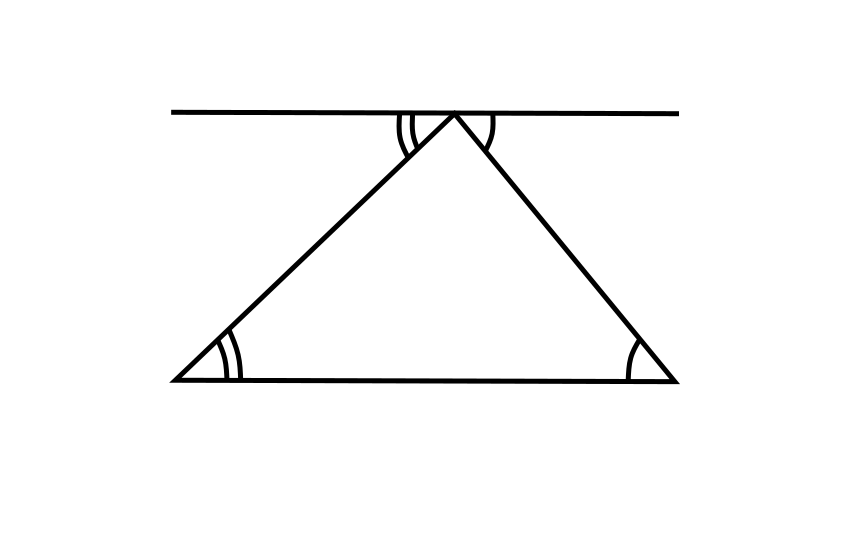
\includegraphics[width=\textwidth]{background/interior-triangle}
         \caption{Interior angles.}
 	 \label{fig:interior-angles}
       \end{subfigure}
         \hspace{1cm}
         \begin{subfigure}[b]{0.25\textwidth}
         \includegraphics[width=\textwidth]{background/exterior-angles-polygon}
         \caption{Exterior angles.}
          \label{fig:exterior-angles}
         \end{subfigure}
		\caption{(a) In the plane, the sum of the interior angles of a triangle is $\pi$
 		and (b) the sum of the exterior angles of a simple
		polygon is $2\pi$. Here
		$\alpha_1+\alpha_2+\alpha_3+\alpha_4+\alpha_5=2\pi$.
 		\label{fig:simple-polygon}}
 \end{figure}

And we have
\begin{corollary}\label{cor:angles}
In the plane, any simple polygon $P$ with $n$ vertices,
the sum of the interior angles of $P$ is $(n-2)\pi$.
\end{corollary}

\begin{proof}
	Consider any simple polygon in the plane $P$ with $n$ vertices. 
	Then $P$ can be triangulated with $n-2$ triangles \cite{orourke_computational_1994}.
	Thus, when we traverse $P$ we go around $n-2$ triangles each contributing
	$\pi$.
\end{proof}

 





On the unit sphere we can determine even more about a polygon 
based on the angles. This is because the sphere is curved.
A triangle on the sphere is shown in \figref{sphere-triangle}.


 \begin{figure}[htb]
         \centering
        \begin{subfigure}[b]{0.35\textwidth}
         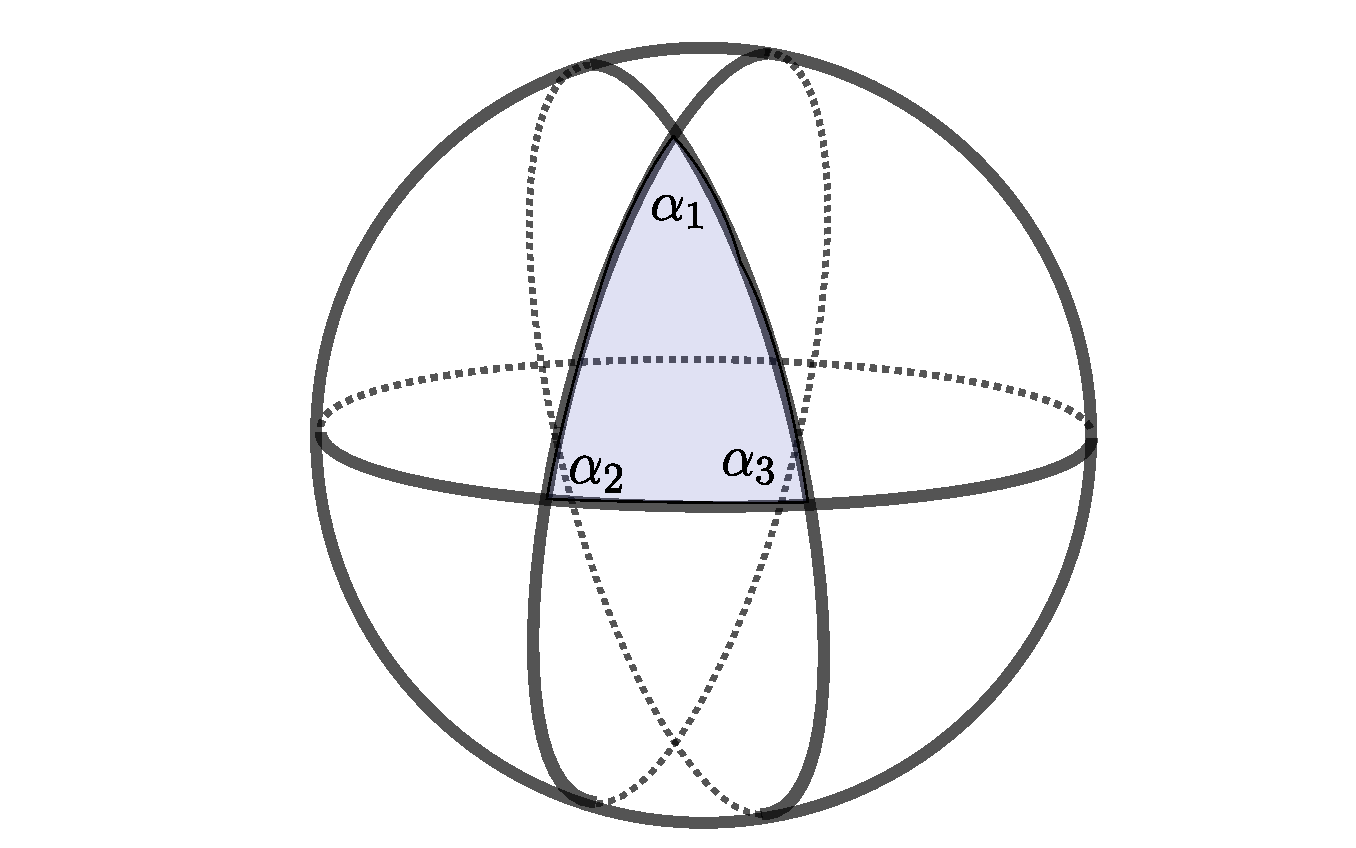
\includegraphics[width=\textwidth]{background/sphere-triangle}
         \caption{Spherical triangle.}
 	 \label{fig:sphere-triangle}
       \end{subfigure}
         \hspace{1cm}
         \begin{subfigure}[b]{0.35\textwidth}
         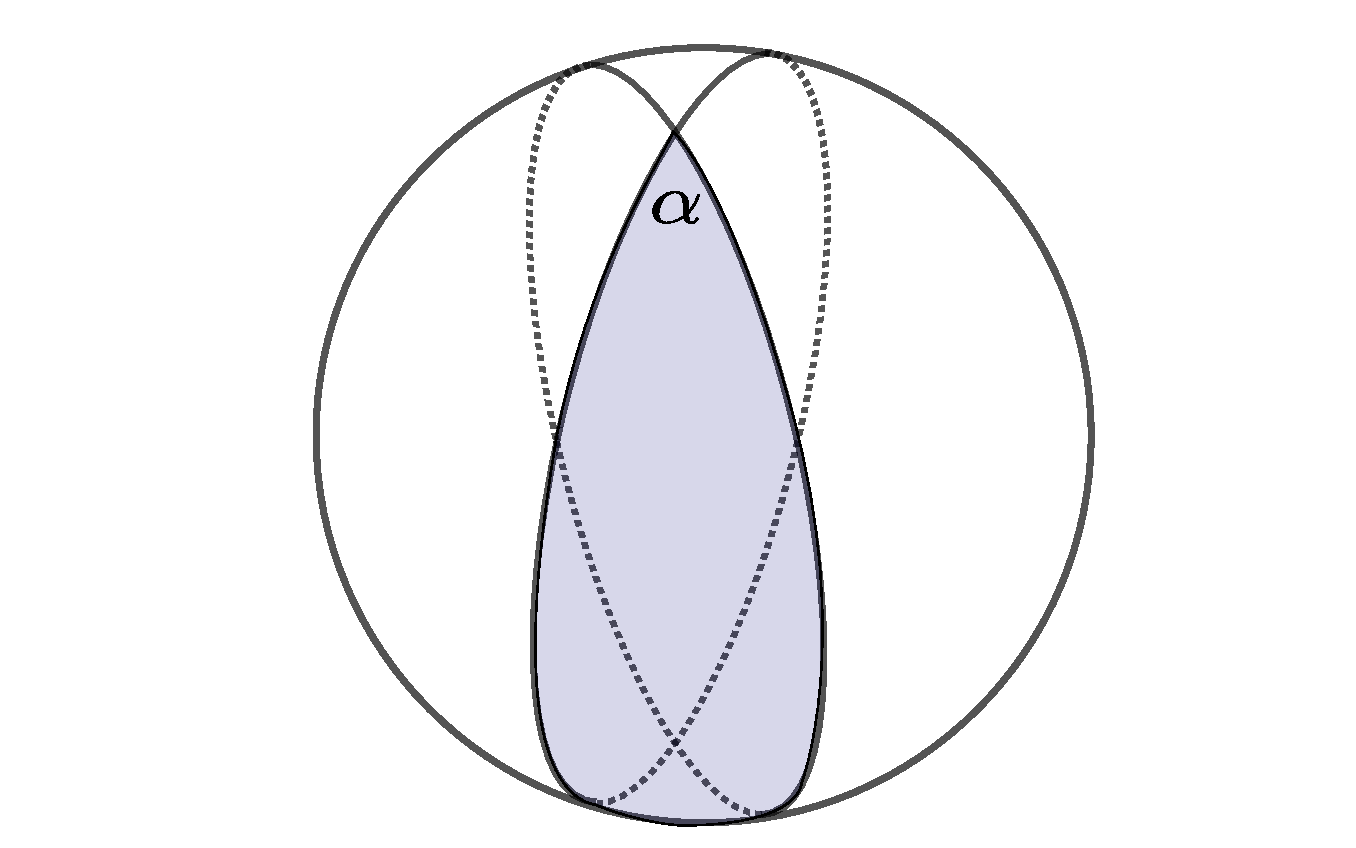
\includegraphics[width=\textwidth]{background/lune}
         \caption{A lune.}
          \label{fig:lune}
         \end{subfigure}
		\caption{(a) A triangle on the sphere.
 		(b) A lune with angle $\alpha$.
 		\label{fig:sphere-lune}}
 \end{figure}
A spherical \EMPH{lune} is the region on a sphere bounded by two half great circles
with angle $\alpha$ the area of a lune is denoted $A(\alpha)$,
 see \figref{lune}.
On the unit sphere, the area of a lune is proportional to $\alpha$. 
If $\alpha=0$ the area is zero and if $\alpha=\pi$ the area is $4\pi$.
We can add the area of two lunes in terms of their angles, 
$A(\alpha_1+\alpha_2)=A(\alpha_1)+A(\alpha_2)$ so $A$ is linear
and  $A(\alpha)=4\alpha.$




The area of a triangle on the sphere is related to the angles.

\begin{lemma}[Area of Spherical Triangle]\label{lem:spherical-triangle}
On the unit sphere, the area of a triangle with interior angles $\alpha_1, \alpha_2, \alpha_3$
is $A=\alpha_1+\alpha_2+\alpha_3-\pi$.
\end{lemma}

\begin{proof}
Any two edges of the the triangle form a lune. The collection of 
all three lunes covers the entire sphere with triangle and the antipodal triangle
are covered three times. The surface area of the unit sphere is $4\pi$.

Thus, $4\pi=2(2\alpha_1+2\alpha_2+2\alpha_3)-6A+2A$
and $A=\alpha_1+\alpha_2+\alpha_3-\pi$.
\end{proof}

As in the plane, any polygon on the sphere with $n$ vertices can be decomposed
into $n-2$ triangles. This gives a formula for the area of a simple polygon
on the sphere with interior angles $\beta_1,\beta_2,\ldots, \beta_n$.

\begin{equation} \label{eqn:sphere-area}
A=(2-n)\pi +\sum_{i=1}^n \beta_i.
\end{equation}








\subsection{Triangulations and The Euler Characteristic}

We assume the reader is familiar with the notions
of topological spaces, manifolds and simplicial complexes.
Most introductory topology texts has contain these definitions \cite{jm08,munkres}.
The applications we will encounter will be a triangulated surfaces
called a \emph{meshs}, in one application the surface will contain its interior.


We denote the set of vertices, edges and faces in a triangulated surface as 
$V, E$ and $F$ respectively.
Let $\partial(V)$ denote vertices on the boundary of a surface and let $V_{int}$ 
denote vertices that are not on the boundary.
See \figref{triangulated-torus} for an example of a triangulated surface.



The \EMPH{Euler Characteristic} for surfaces $\chi$ is the 
the number of vertices minus the number of edges plus  the number of faces, $\chi=|V|-|E|+|F|.$
In higher dimensions, for a triangulated space $X$ the Euler characteristic is 
$\chi(X)=k_0-k_1+k_2-k_3+\ldots$ where $k_n$ is the number of simplices of dimension $n.$
The Euler characteristic is a topological invariant of a space
and does not depend on the choice of triangulation.


Two dimensional spheres $\Sp^2$ and two dimensional disk $D^2$ 
will be used in our applications.
For the sphere, we have $\chi(\Sp^2)=2$ 
several proofs of this can be found on David Eppstein's website \cite{eppstein-proofs}.
For the disk, $\chi(D^2)=1$. The disk can be triangulated by
a single solid triangle with three vertices, three edges and one face.



The \EMPH{genus} of a surface is the maximum number of closed simple
non-intersecting curves that can be drawn in the surface without separating
the surface.
The torus in \figref{triangulated-torus} has genus one.
By the classification of surfaces \cite{munkres}, the Euler characteristic or an orientable surface
is determined by its genus with $\chi=2-2g$.



\begin{figure}[htb]
\centering
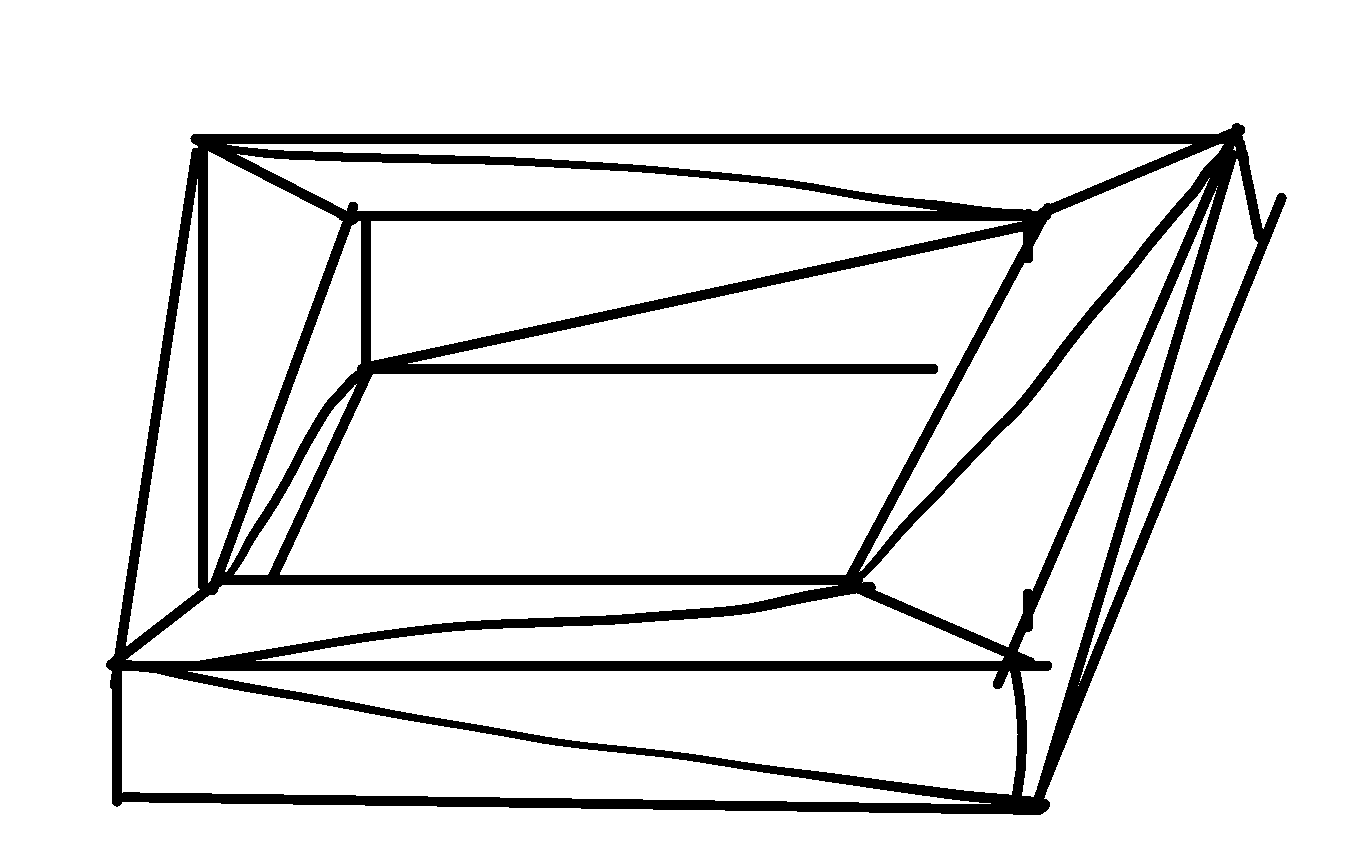
\includegraphics[width=.3\textwidth]{curvature/triangulated-torus}
\caption{A triangulation of the torus.}
\label{fig:triangulated-torus}
\end{figure}

\subsection{Curvature}




There are several ways to define curvature in the discrete setting \cite{Crane:2013}.
For a piecewise linear curve in $\R^2$, what properties should we
require of our definition of curvature at a vertex?
If two segments are colinear, the curvature should be zero.
There are two possible angles we could use to describe the
curvature and they are supplementary, see \figref{2d-curvature}.

\begin{figure}[htb]
\centering
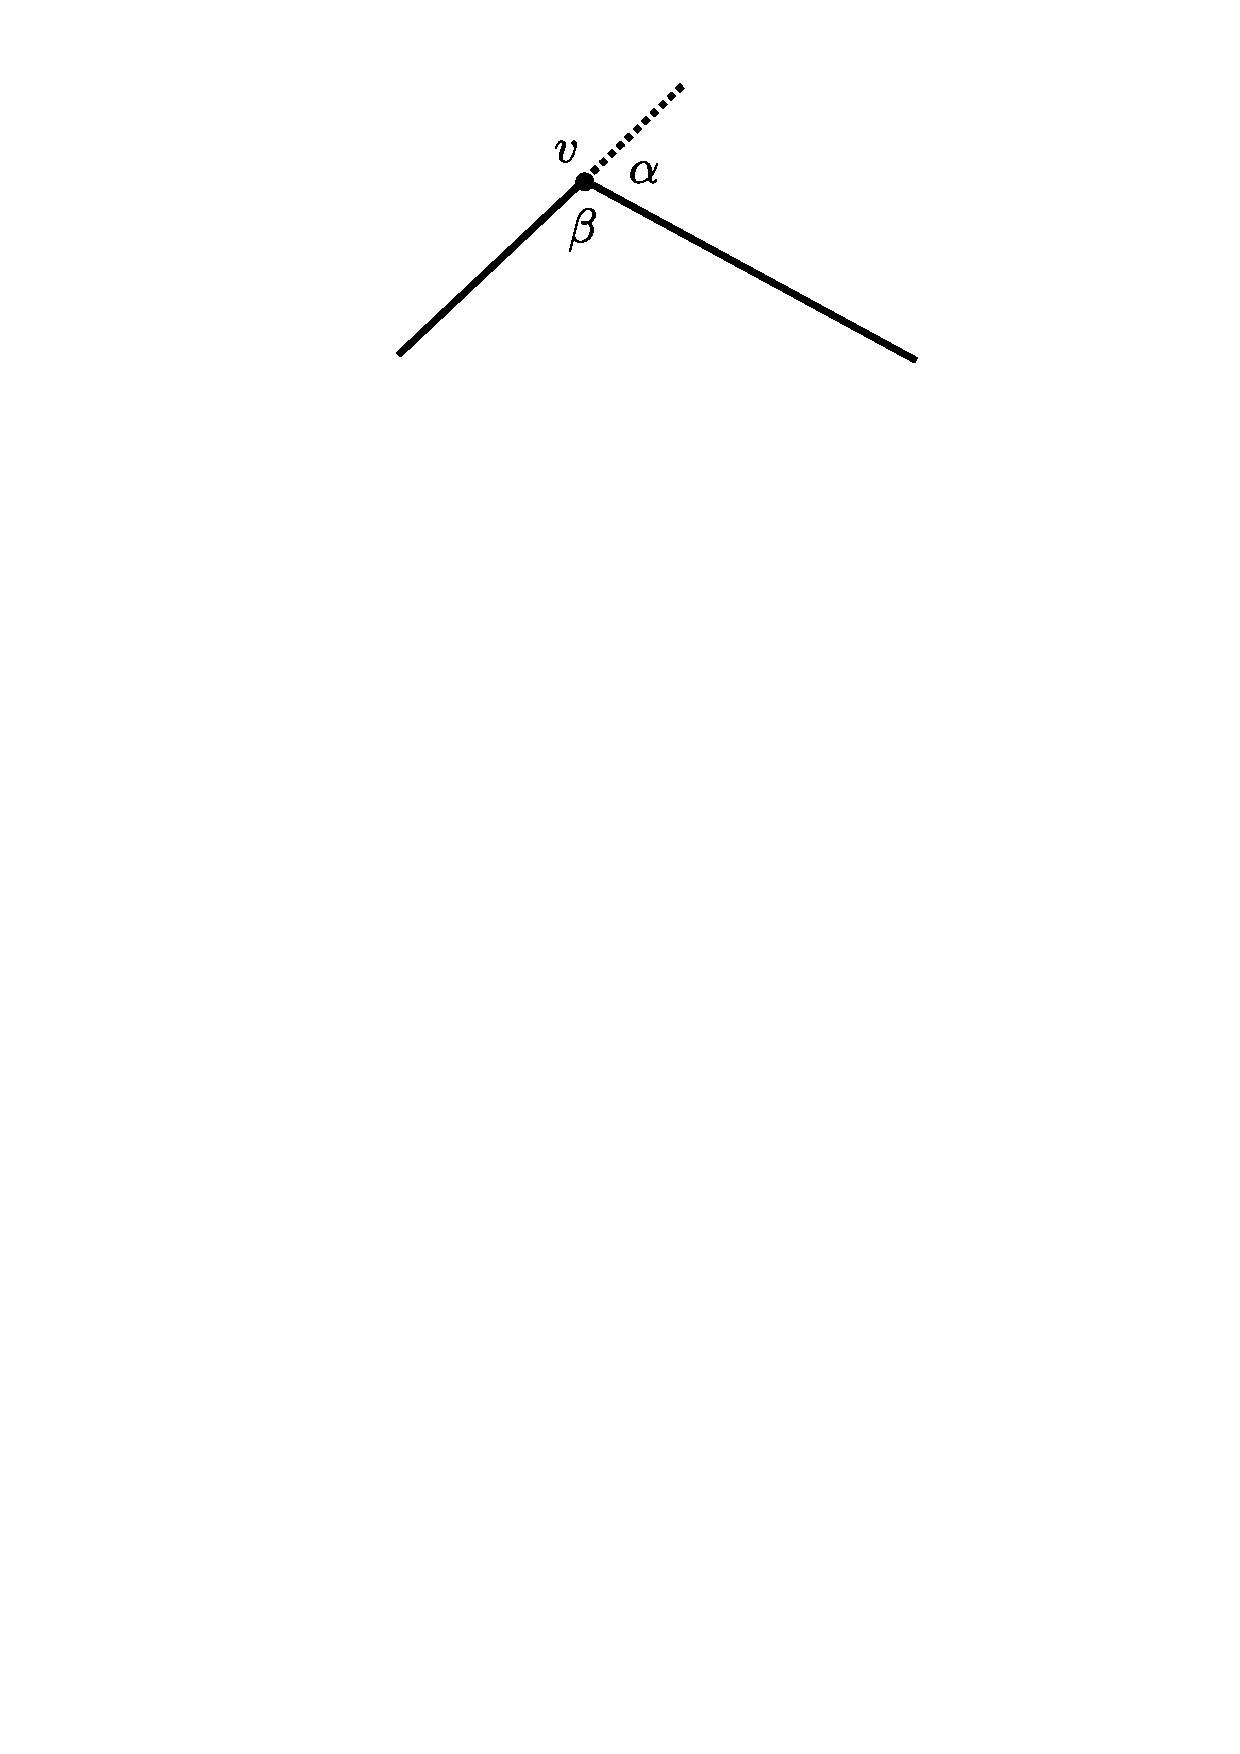
\includegraphics[width=.3\textwidth]{background/2d-curvature}
\caption{A vertex $v$ in a piecewise linear curve.
We can measure the curvature at $v$ in terms the angle
$\alpha$ or $\beta$. We want straight lines to have
zero curvature and the curvature to decrease as $\alpha$
increases, so, we define the curvature to be $\pi-\alpha$.
}
\label{fig:2d-curvature}
\end{figure}


For a vertex in a discrete surface, the Gaussian curvature is defined as
follows

\begin{definition}[Discrete Gaussian curvature]\label{def:discrete-curvature-vertex}

The discrete \EMPH{Gaussian curvature} at a vertex $v$ is the area on the unit sphere bounded by a spherical polygon whose vertices are the unit normals of the faces around $v$.

\end{definition}


\begin{figure}[htb]
\centering
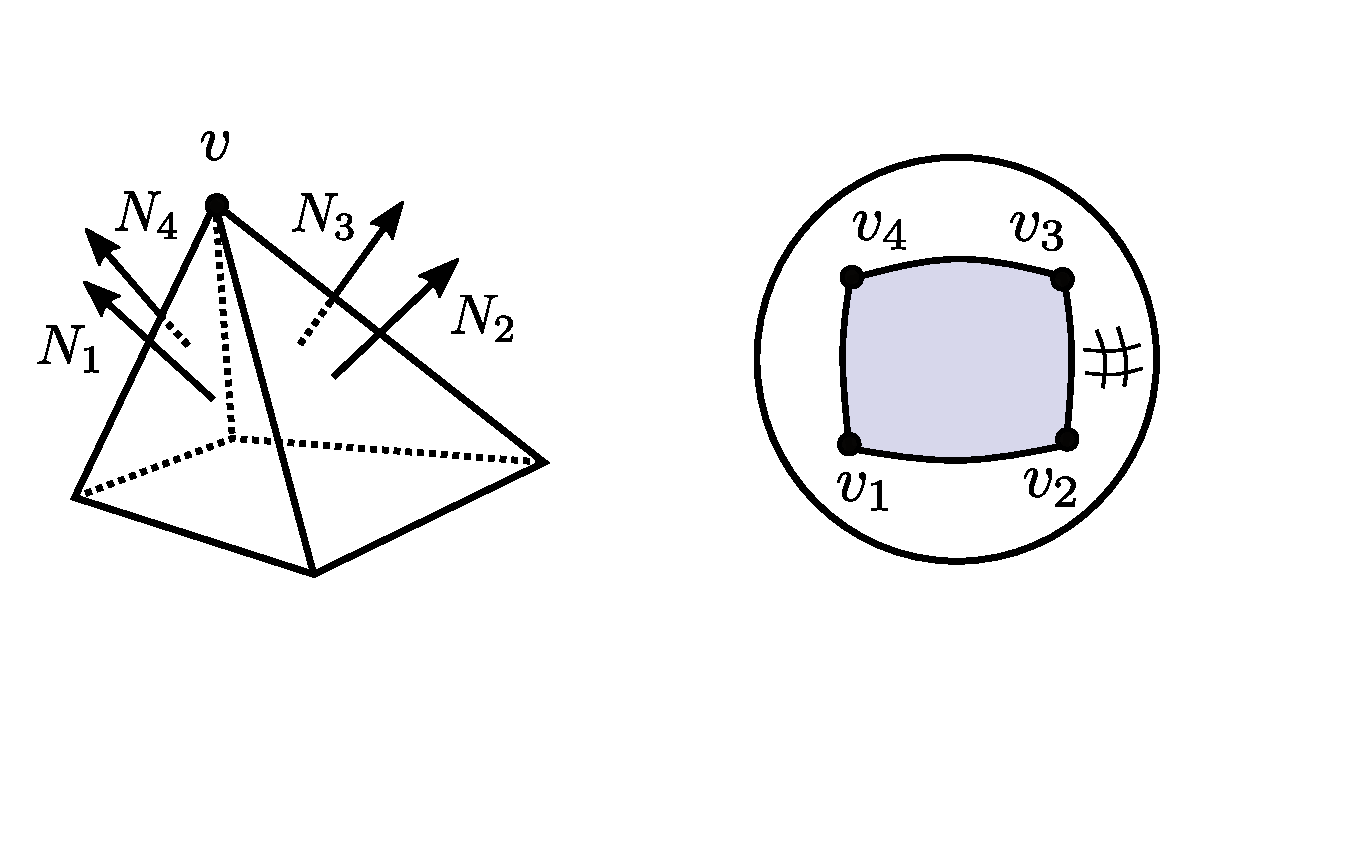
\includegraphics[width=.5\textwidth]{curvature/discrete-curvature}
\caption{Consider the vertex $v$ on the left. The curvature of $v$
is the area on the sphere shown on the right. We rotated the sphere
in order to see the entire polygon.}
\label{fig:discrete-curvature}
\end{figure}


\eqnref{sphere-area} gives a formula for computing the curvature at a vertex, provided
we know the interior angles of the polygon on the sphere.
The interior angles of the polygon $\beta_i$ on the sphere are supplementary to
the angle $\alpha_i$ incident to $v$ in the surface

\begin{equation} \label{eqn:switcheroo}
\beta=\pi-\alpha.
\end{equation}
See \figref{switcheroo} for an example.




\begin{figure}[htb]
\centering
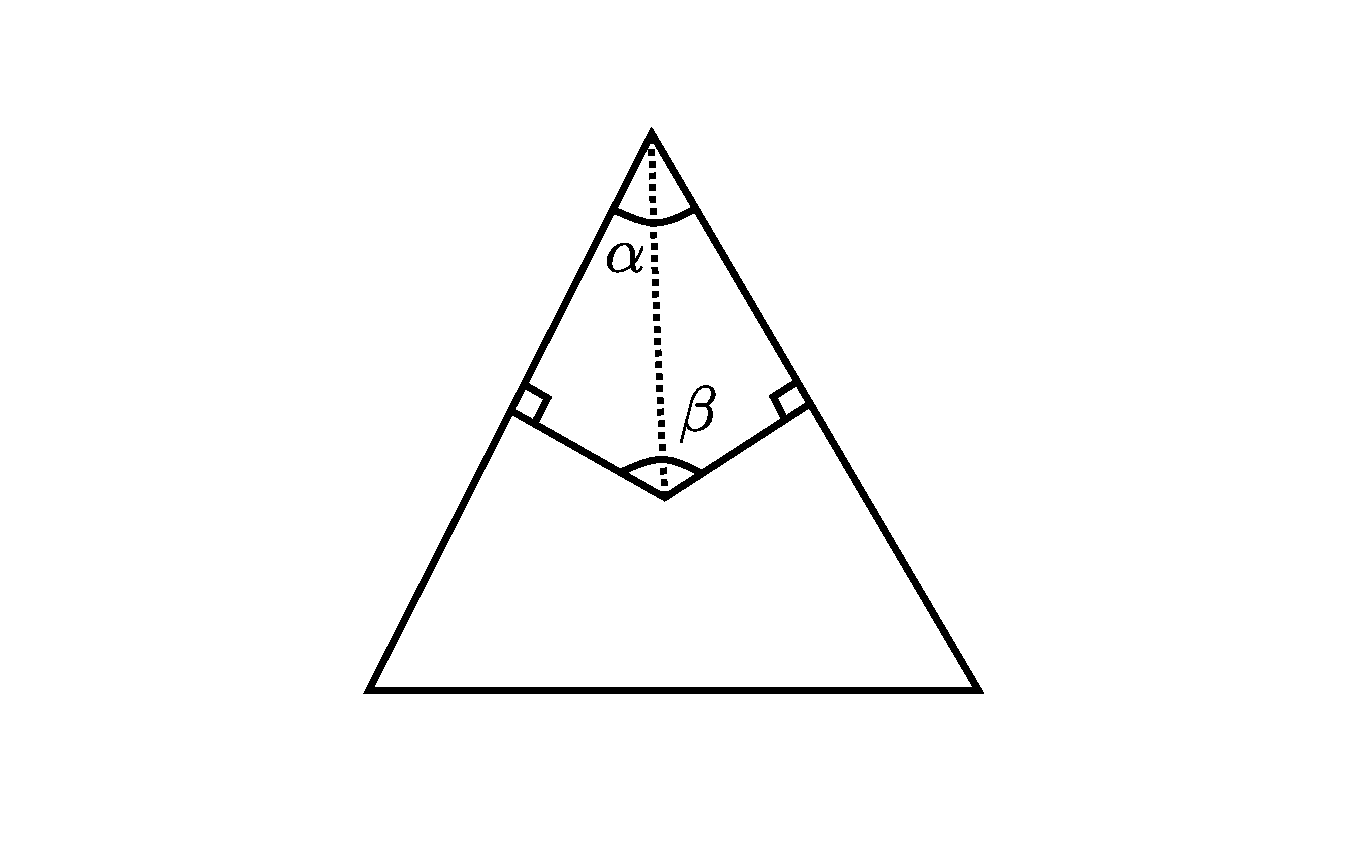
\includegraphics[width=.3\textwidth]{background/switch-angles}
\caption{The relationship between the angles incident to a vertex and
the interior angles of the area polygon on the sphere.}
\label{fig:switcheroo}
\end{figure}




This gives a convenient formula for computing the curvature at a vertex.
The \EMPH{angle defect} at a vertex $d(v)$ is the difference between $2\pi$ and
the sum of the incident angles.  Let $F_v$ denote the faces containing $v$  
and let $\alpha_f$  denote the interior  angle of face $f$ at $v$, then
$$d(v):=2\pi -\sum_{f\in F_v}\alpha_f.$$

Since $\beta_i=\pi-\alpha_i$, we have the Gaussian curvature at $v$
is 
$$k(v)=2\pi -n\pi+\sum_{i}^n \beta_i=2\pi-n\pi +n\pi -\sum_i^n\alpha_i=d(v)$$
 and the
 angle defect is equal to the discrete curvature in \defref{discrete-curvature-vertex}.


For a vertex $v$ on the boundary of a surface, we define the the curvature
of $v$  to be 
$$k_{\partial}(v)= \pi-\sum_{f\in F_vi}\alpha_f.$$
Notice that if $v$ lies on a straight line, then $\sum_{i}\alpha_f=\pi$
and the curvature is $0$ as we would expect.
For historical reasons,  we write $k_g(v)=k_{\partial}(v)$
where the subscript $g$ refers to geodesic curature.
Curvature is defined more naturally in the continuous setting,
discrete curvature is an oxymoron.  See do Carmo \cite{doc76} for an introduction.
The juxtaposition between the continuous and discrete versions of the theorem
is pleasing.



Putting all of these variables together gives \thmref{g-b}.
The  Gauss-Bonnet theorem is  telling us, if we add up curvature
at each vertex the sum will be $2\pi$ times to Euler characteristic.
If we can compute the curvature at every vertex then we can use the theorem
to learn global topological information.
Conversely, if we know the Euler characteristic we can learn about the curvature
at individual points.
